\begin{frame}{Closed-World Assumption and the Open-Set Problem}
  \begin{columns}[T,onlytextwidth]
    \column{0.58\textwidth}
      \begin{itemize}\footnotesize\itemsep0.35em
        \item \textbf{Closed world:} a classifier trained on $K$ known classes assumes every test image is \textbf{in-distribution (ID)}; shown an unseen class, it still picks one of its $K$ labels.
        \item \textbf{Open-set recognition (OSR)} (Scheirer et al., TPAMI 2013): classify the known classes and reject the unknown ones; ``the classifier must also support rejection.''
        \item \textbf{Out-of-distribution (OOD) detection}: flag inputs whose class is outside the training label set (\textbf{semantic shift}). Yang et al.\ (IJCV 2024) treat it and OSR as one problem.
        \item Related tasks: anomaly, novelty and outlier detection. Autoencoder reconstruction error is an anomaly score.
        \item \textbf{Unlike covariate shift:} ImageNet-R and ImageNet-Sketch are covariate shift (same classes, new style), scored by accuracy; under semantic shift the right answer is \textit{unknown}.
      \end{itemize}
    \column{0.40\textwidth}
      \centering
      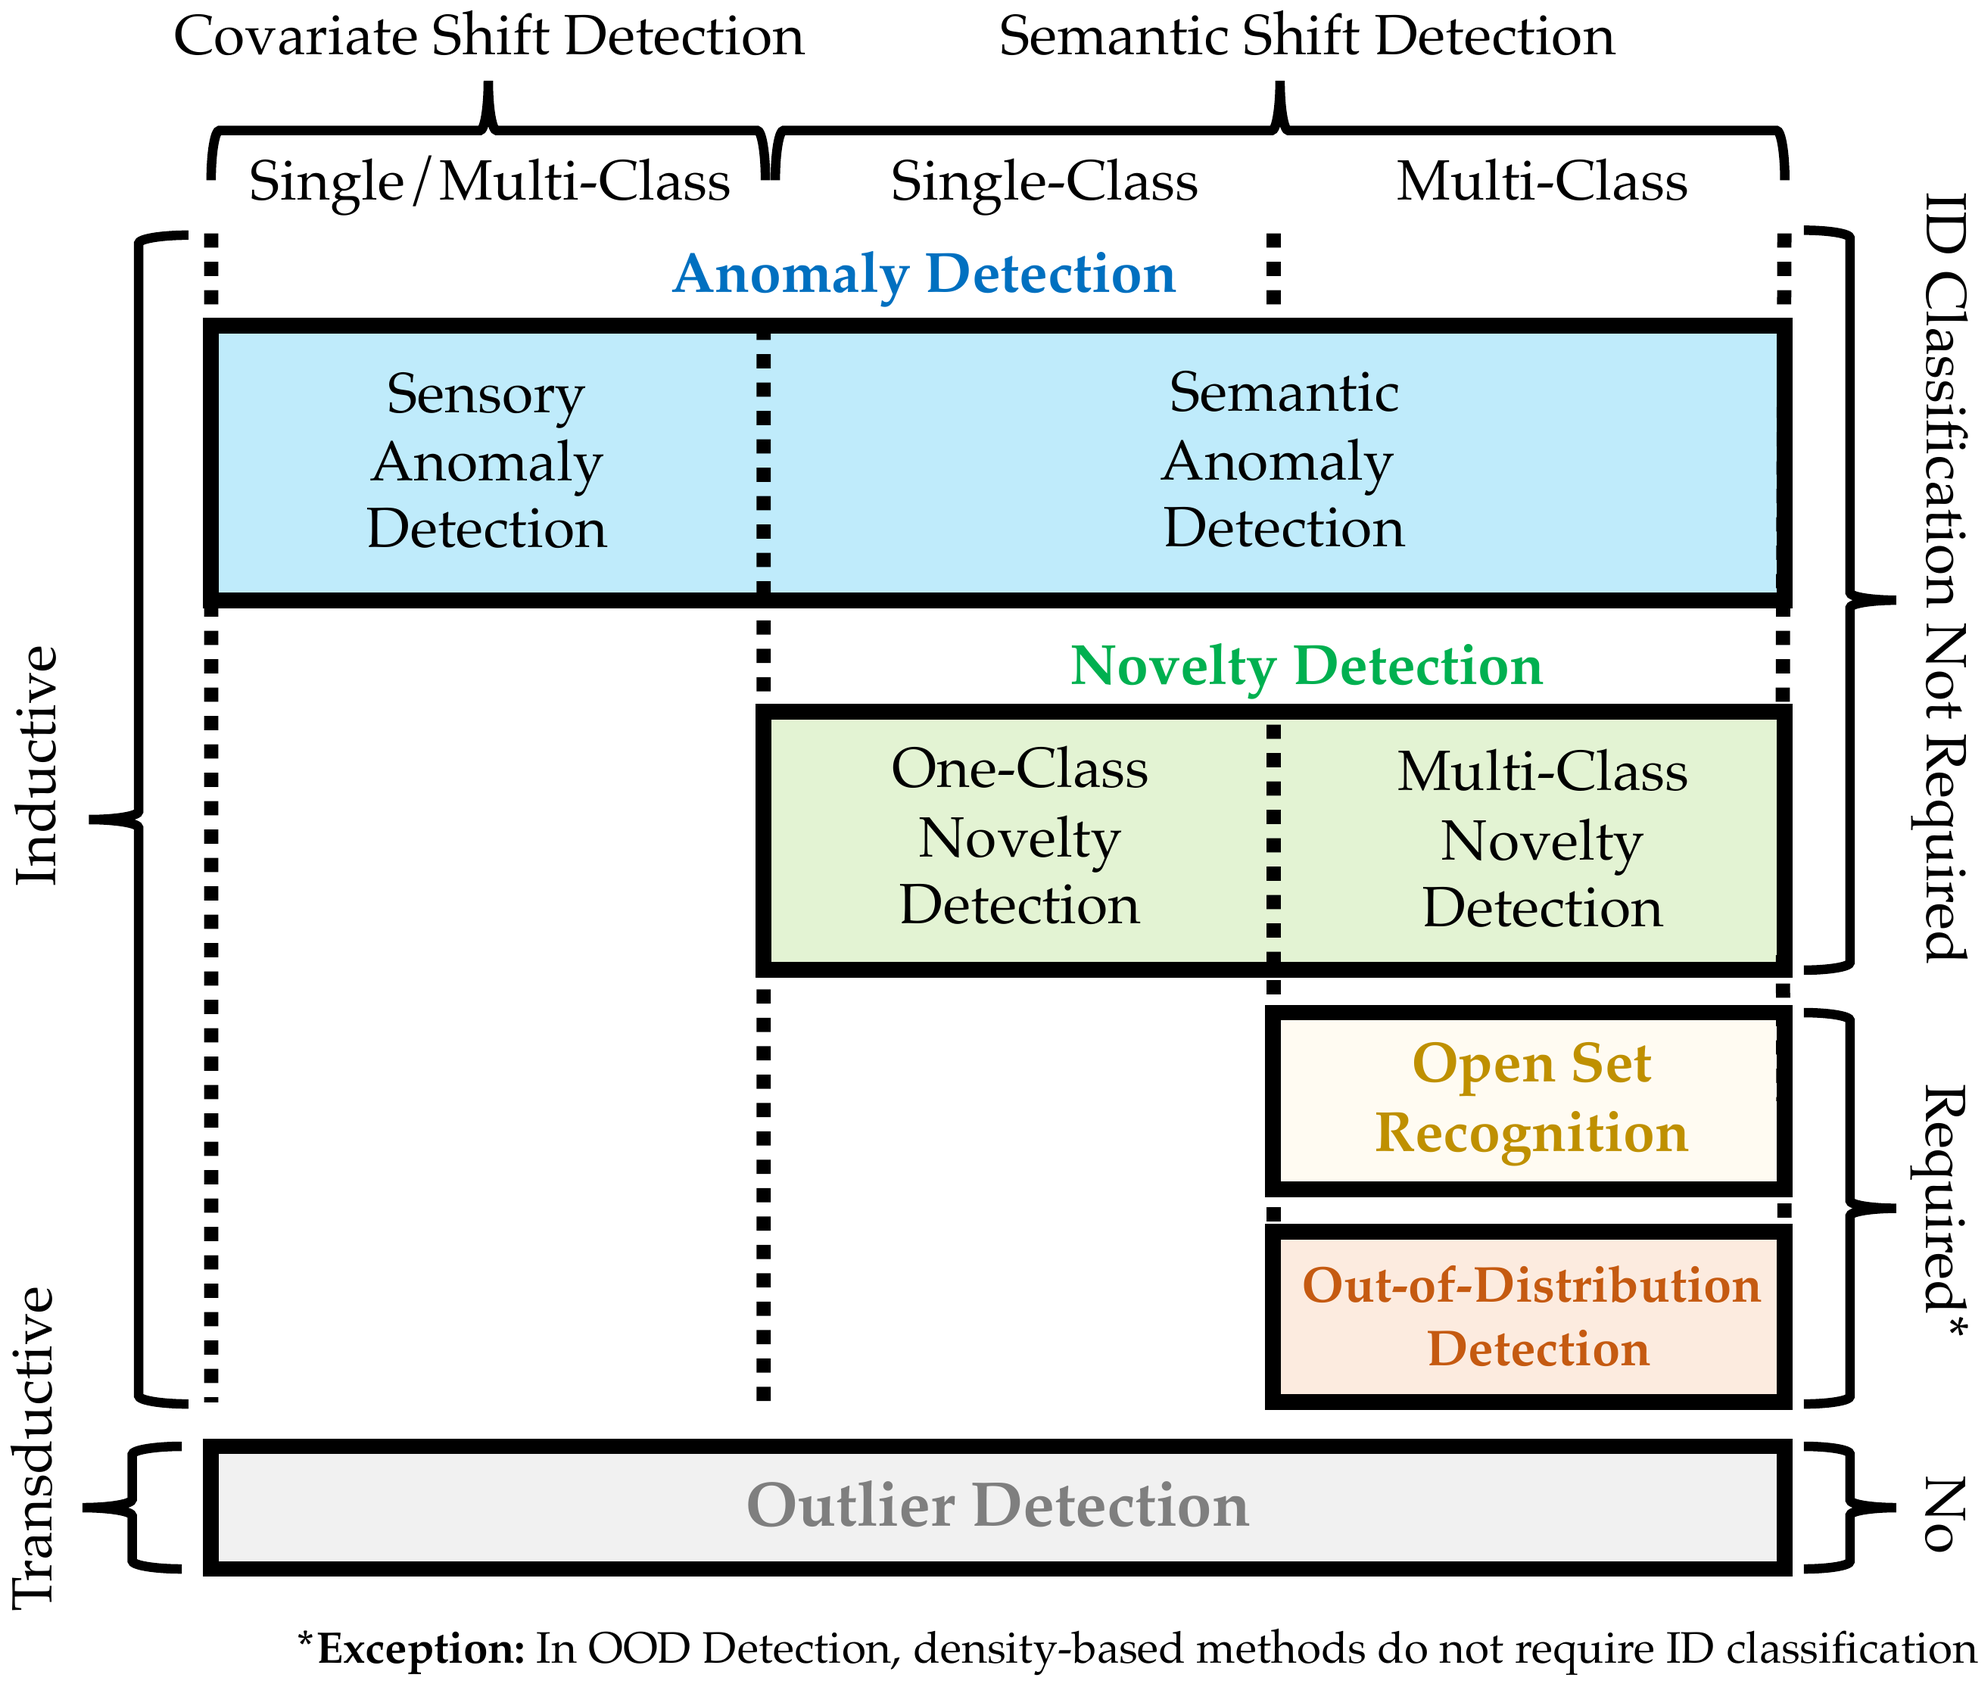
\includegraphics[width=\linewidth,height=0.66\textheight,keepaspectratio]{images/image-recognition/genood_fig1_taxonomy.png}\\[0.2em]
      {\scriptsize Tasks sorted by shift type, number of ID classes, and whether ID classification is required. Yang et al., ``Generalized Out-of-Distribution Detection: A Survey,'' IJCV 2024, \href{https://arxiv.org/abs/2110.11334v3}{arXiv:2110.11334v3}, Figure~1.\par}
  \end{columns}
\end{frame}

\begin{frame}{Softmax Confidence Fails Far From the Data}
  \begin{columns}[T,onlytextwidth]
    \column{0.52\textwidth}
      \begin{itemize}\footnotesize\itemsep0.35em
        \item \textbf{Maximum softmax probability (MSP)} baseline (Hendrycks and Gimpel, ICLR 2017): score $s(x)=\max_k p(k\mid x)$, with $p(k\mid x)$ the softmax output for class $k$. Correctly classified images tend to score higher than misclassified and OOD images.
        \item The value alone misleads: their MNIST classifier gives Gaussian noise a mean MSP of 91\%.
        \item \textbf{Cause} (Hein et al., CVPR 2019): a ReLU network is piecewise affine, and its outer linear regions extend to infinity. For almost every input $x$,
        \[ \lim_{\alpha\to\infty}\, \max_k \frac{e^{z_k(\alpha x)}}{\sum_{j=1}^{K} e^{z_j(\alpha x)}} = 1, \]
        where $z_k$ is the logit of class $k$ and $\alpha>0$ scales the input away from the data.
        \item Softmax temperature cannot undo this. Uniform noise scaled by a median $\alpha=8.1$ already gets 99.9\% confidence from their CIFAR-10 model.
      \end{itemize}
    \column{0.46\textwidth}
      \centering
      \vspace{0.3em}
      \resizebox{\linewidth}{!}{%
      \begin{tikzpicture}[font=\sffamily\scriptsize, >=latex]
        \fill[green!14] (0.83,0) rectangle (1.38,2.8);
        \node[green!40!black] at (1.1,0.3) {data};
        \draw[gray, dashed] (0,0.933) -- (5.5,0.933);
        \draw[gray, dashed] (0,2.8) -- (5.5,2.8);
        \draw[->] (0,0) -- (5.85,0) node[right] {$\alpha$};
        \draw[->] (0,0) -- (0,3.1) node[above] {$\max_k p(k\mid \alpha x)$};
        \foreach \x/\l in {0/0, 1.1/1, 2.2/2, 3.3/3, 4.4/4, 5.5/5}
          \draw (\x,0) -- (\x,-0.06) node[below] {\l};
        \draw (0,0.933) -- (-0.06,0.933) node[left] {$1/K$};
        \draw (0,2.8) -- (-0.06,2.8) node[left] {1};
        \draw[very thick, KAred] plot coordinates {(0.00,0.93) (0.28,1.35) (0.55,1.76) (0.83,2.11) (1.10,2.36) (1.38,2.53) (1.65,2.64) (1.93,2.70) (2.20,2.74) (2.48,2.77) (2.75,2.78) (3.03,2.79) (3.30,2.79) (3.58,2.80) (3.85,2.80) (4.12,2.80) (4.40,2.80) (4.68,2.80) (4.95,2.80) (5.23,2.80) (5.50,2.80)};
        \draw[very thick, KAUSTblue] plot coordinates {(0.00,1.92) (0.28,2.11) (0.55,2.25) (0.83,2.34) (1.10,2.36) (1.38,2.34) (1.65,2.25) (1.93,2.11) (2.20,1.92) (2.48,1.69) (2.75,1.47) (3.03,1.29) (3.30,1.15) (3.58,1.06) (3.85,1.00) (4.12,0.97) (4.40,0.95) (4.68,0.94) (4.95,0.94) (5.23,0.93) (5.50,0.93)};
        \node[KAred, anchor=north east] at (5.5,2.7) {ReLU network: $\to 1$};
        \node[KAUSTblue, anchor=south east] at (5.5,1.2) {RBF-type: $\to 1/K$};
      \end{tikzpicture}}\\[0.3em]
      {\scriptsize Toy model with $K=3$ along the ray $\alpha x$: affine logits $\alpha\,(3,1,0)$, as inside one linear region of a ReLU network (red), and radial-basis-function (RBF) logits $e^{-(\alpha-1)^2/2}\,(3,1,0)$ that decay away from the data (blue). Both give 0.84 at the training point $\alpha=1$; far away the ReLU confidence goes to 1, while the RBF-type confidence returns to $1/K$, as in Hein et al.'s Theorem~3.2.\par}
  \end{columns}
\end{frame}

\begin{frame}{Evaluating a Detector: AUROC, FPR95, AUPR, OSCR}
  \begin{columns}[T,onlytextwidth]
    \column{0.52\textwidth}
      \begin{itemize}\footnotesize\itemsep0.3em
        \item \textbf{Detector:} score $s(x)$ (higher for ID), threshold $\lambda$: predict a class if $s(x)\geq\lambda$, else \textit{unknown}; $\lambda$ is set on ID data, e.g.\ to accept 95\% of ID images.
        \item \textbf{Convention: ID is positive.} TPR is the share of ID images accepted, FPR of OOD images accepted; the ROC curve plots TPR against FPR as $\lambda$ sweeps.
        \item \textbf{AUROC:} area under the ROC curve: the probability that a random ID image outscores a random OOD image (50\% is chance).
        \item \textbf{FPR95:} the FPR at the $\lambda$ that accepts 95\% of ID images; lower is better.
        \item \textbf{AUPR-In/Out:} area under the precision-recall curve, ID or OOD positive; depends on the ID:OOD ratio.
        \item \textbf{OSCR curve} (open-set classification rate; Dhamija et al., NeurIPS 2018): known-class images accepted \emph{and} correctly classified, against FPR.
      \end{itemize}
    \column{0.46\textwidth}
      \centering
      \resizebox{\linewidth}{!}{%
      \begin{tikzpicture}[font=\sffamily\scriptsize, >=latex]
        \begin{scope}[yshift=3.1cm]
          \fill[orange!30] (2.21,0) -- (2.21,0.95) -- plot coordinates {(2.27,0.93) (2.45,0.84) (2.62,0.72) (2.80,0.58) (2.97,0.44) (3.15,0.31) (3.32,0.21) (3.50,0.13) (3.67,0.08) (3.85,0.04) (4.02,0.02) (4.20,0.01) (4.38,0.00)} -- cycle;
          \draw[thick, gray] plot[smooth] coordinates {(0.00,0.01) (0.17,0.02) (0.35,0.04) (0.52,0.08) (0.70,0.13) (0.88,0.21) (1.05,0.31) (1.22,0.44) (1.40,0.58) (1.57,0.72) (1.75,0.84) (1.92,0.93) (2.10,0.96) (2.27,0.93) (2.45,0.84) (2.62,0.72) (2.80,0.58) (2.97,0.44) (3.15,0.31) (3.32,0.21) (3.50,0.13) (3.67,0.08) (3.85,0.04) (4.02,0.02) (4.20,0.01) (4.38,0.00) (5.60,0.00)};
          \draw[thick, KAUSTblue] plot[smooth] coordinates {(0.00,0.00) (1.05,0.00) (1.22,0.01) (1.40,0.02) (1.57,0.04) (1.75,0.07) (1.92,0.12) (2.10,0.19) (2.27,0.29) (2.45,0.41) (2.62,0.55) (2.80,0.70) (2.97,0.82) (3.15,0.92) (3.32,0.96) (3.50,0.94) (3.67,0.87) (3.85,0.75) (4.02,0.61) (4.20,0.47) (4.38,0.33) (4.55,0.23) (4.72,0.14) (4.90,0.09) (5.07,0.05) (5.25,0.03) (5.42,0.01) (5.60,0.01)};
          \draw[->] (0,0) -- (5.85,0) node[right] {$s(x)$};
          \draw[KAred, dashed, thick] (2.21,0) -- (2.21,1.05) node[above] {$\lambda$};
          \node[gray!70!black] at (0.75,0.6) {OOD};
          \node[KAUSTblue] at (4.75,0.6) {ID};
        \end{scope}
        \begin{scope}[xshift=0.75cm]
          \fill[blue!12] (0,0) -- plot coordinates {(0.000,0.000) (0.000,0.059) (0.001,0.142) (0.004,0.299) (0.012,0.551) (0.036,0.896) (0.059,1.094) (0.093,1.300) (0.142,1.506) (0.210,1.704) (0.299,1.887) (0.413,2.049) (0.551,2.187) (0.713,2.301) (0.896,2.390) (1.094,2.458) (1.140,2.470) (1.300,2.507) (1.506,2.541) (1.887,2.579) (2.301,2.596) (2.600,2.600)} -- (2.6,0) -- cycle;
          \draw (0,0) rectangle (2.6,2.6);
          \draw[gray, dashed] (0,0) -- (2.6,2.6);
          \draw[thick, KAUSTblue] plot coordinates {(0.000,0.000) (0.000,0.059) (0.001,0.142) (0.004,0.299) (0.012,0.551) (0.036,0.896) (0.059,1.094) (0.093,1.300) (0.142,1.506) (0.210,1.704) (0.299,1.887) (0.413,2.049) (0.551,2.187) (0.713,2.301) (0.896,2.390) (1.094,2.458) (1.140,2.470) (1.300,2.507) (1.506,2.541) (1.887,2.579) (2.301,2.596) (2.600,2.600)};
          \draw[KAred, dashed] (0,2.47) -- (1.14,2.47) -- (1.14,0);
          \fill[KAred] (1.14,2.47) circle (1.6pt);
          \node[left] at (0,2.47) {0.95};
          \node[below] at (0,0) {0};
          \node[below] at (1.14,0) {0.44};
          \node[below] at (2.6,0) {1};
          \node at (1.3,-0.62) {FPR (OOD accepted)};
          \node[rotate=90] at (-0.45,1.2) {TPR (ID accepted)};
          \node[align=left, anchor=west] at (2.75,1.55) {AUROC $=0.90$\\(blue area)};
          \node[KAred, anchor=west] at (2.75,0.75) {FPR95 $=0.44$};
        \end{scope}
      \end{tikzpicture}}\\[0.3em]
      {\scriptsize Binormal example (ID scores $\mathcal{N}(1.8,1)$, OOD scores $\mathcal{N}(0,1)$): the OOD mass above $\lambda$ (orange) is the FPR95; the blue area is the AUROC.\par}
  \end{columns}
\end{frame}

\begin{frame}{Logit Scores: MSP, MaxLogit, and Energy}
  \begin{columns}[T,onlytextwidth]
    \column{0.52\textwidth}
      \begin{itemize}\footnotesize\itemsep0.3em
        \item Notation: penultimate features $h(x)\in\mathbb{R}^D$, logits $z(x)=W h(x)+b\in\mathbb{R}^K$; no retraining.
        \item \textbf{MaxLogit} (maximum logit score, MLS; Hendrycks et al., ICML 2022): $s(x)=\max_k z_k(x)$. With many similar classes the softmax spreads its mass and MSP rejects hard ID images; ResNet-50 on ImageNet: FPR95 44.2 (MSP) to 35.8.
        \item \textbf{Energy} (Liu et al., NeurIPS 2020), with temperature $T$ (they use $T=1$):
        \[ E(x) = -T \log \sum_{k=1}^{K} e^{z_k(x)/T}, \qquad s(x) = -E(x). \]
        At $T=1$, $\max_k z_k \leq -E \leq \max_k z_k + \log K$: a smooth MaxLogit.
        \item \textbf{Why MSP is biased} ($T=1$): $\log \max_k p(k\mid x) = \max_k z_k(x) + E(x)$; ID inputs raise the first term and lower the second, so they partly cancel. CIFAR-10 WideResNet (a wider, shallower ResNet), six OOD sets: FPR95 51.04 (MSP) to 33.01 (energy).
      \end{itemize}
    \column{0.46\textwidth}
      \centering
      \vspace{0.6em}
      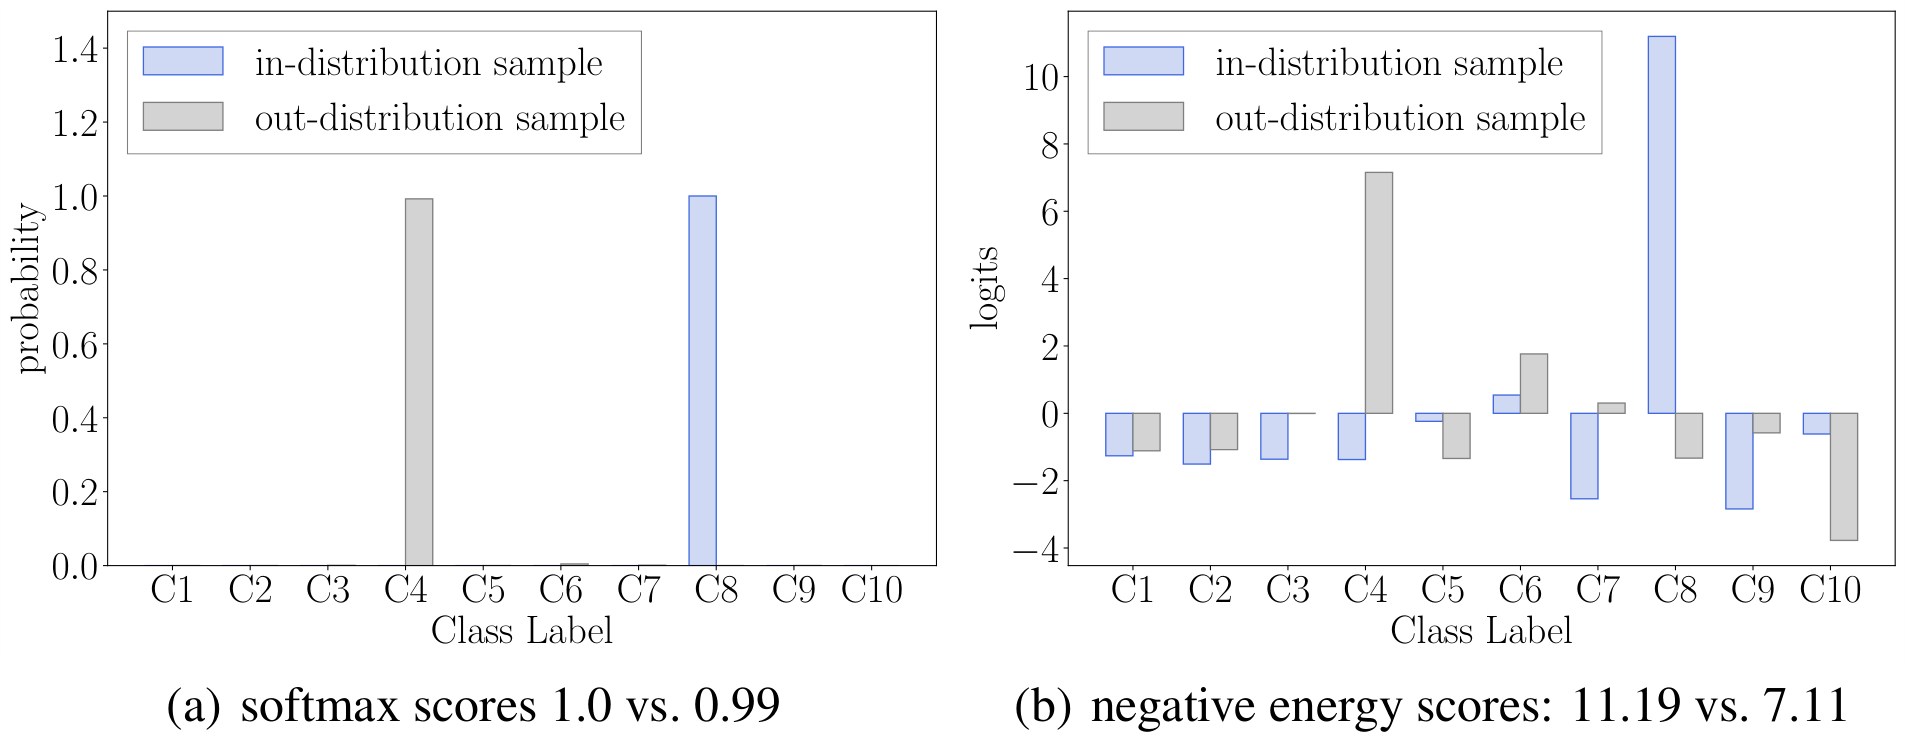
\includegraphics[width=\linewidth,height=0.42\textheight,keepaspectratio]{images/image-recognition/energyood_fig2_softmax_vs_energy.png}\\[0.2em]
      {\scriptsize One CIFAR-10 image (ID) and one SVHN street-number image (OOD) on a CIFAR-10 WideResNet: MSP 1.0 vs 0.99, negative energy 11.19 vs 7.11. Liu et al., ``Energy-based Out-of-distribution Detection,'' NeurIPS 2020, \href{https://arxiv.org/abs/2010.03759v4}{arXiv:2010.03759v4}, Figure~2.\par}
  \end{columns}
\end{frame}

\begin{frame}{Feature-Space Scores: Mahalanobis and Deep k-NN}
  \begin{columns}[T,onlytextwidth]
    \column{0.50\textwidth}
      \begin{itemize}\footnotesize\itemsep0.3em
        \item \textbf{Mahalanobis} (Lee et al., NeurIPS 2018): class means $\mu_c$ and one shared covariance $\Sigma$ of the training features $h(x)$, then
        \[ s(x)=\max_{c}\, -\big(h(x)-\mu_c\big)^{\top}\Sigma^{-1}\big(h(x)-\mu_c\big). \]
        It assumes Gaussian classes: weak on ResNet-50 (table), AUROC 96.02 on ViT-B/16 (other OOD sets; Wang et al., CVPR 2022).
        \item \textbf{Deep $k$-NN} (Sun et al., ICML 2022): $s(x)=-\|u-u_{(k)}\|_2$, with $u=h(x)/\|h(x)\|_2$ and $u_{(k)}$ its $k$-th nearest normalised training feature. No distribution assumption; the threshold uses ID data only.
        \item Approximate nearest-neighbour search keeps $k$-NN fast. On SupCon features, which form compact classes, its FPR95 drops from 54.68 to 38.47.
      \end{itemize}
    \column{0.48\textwidth}
      \centering
      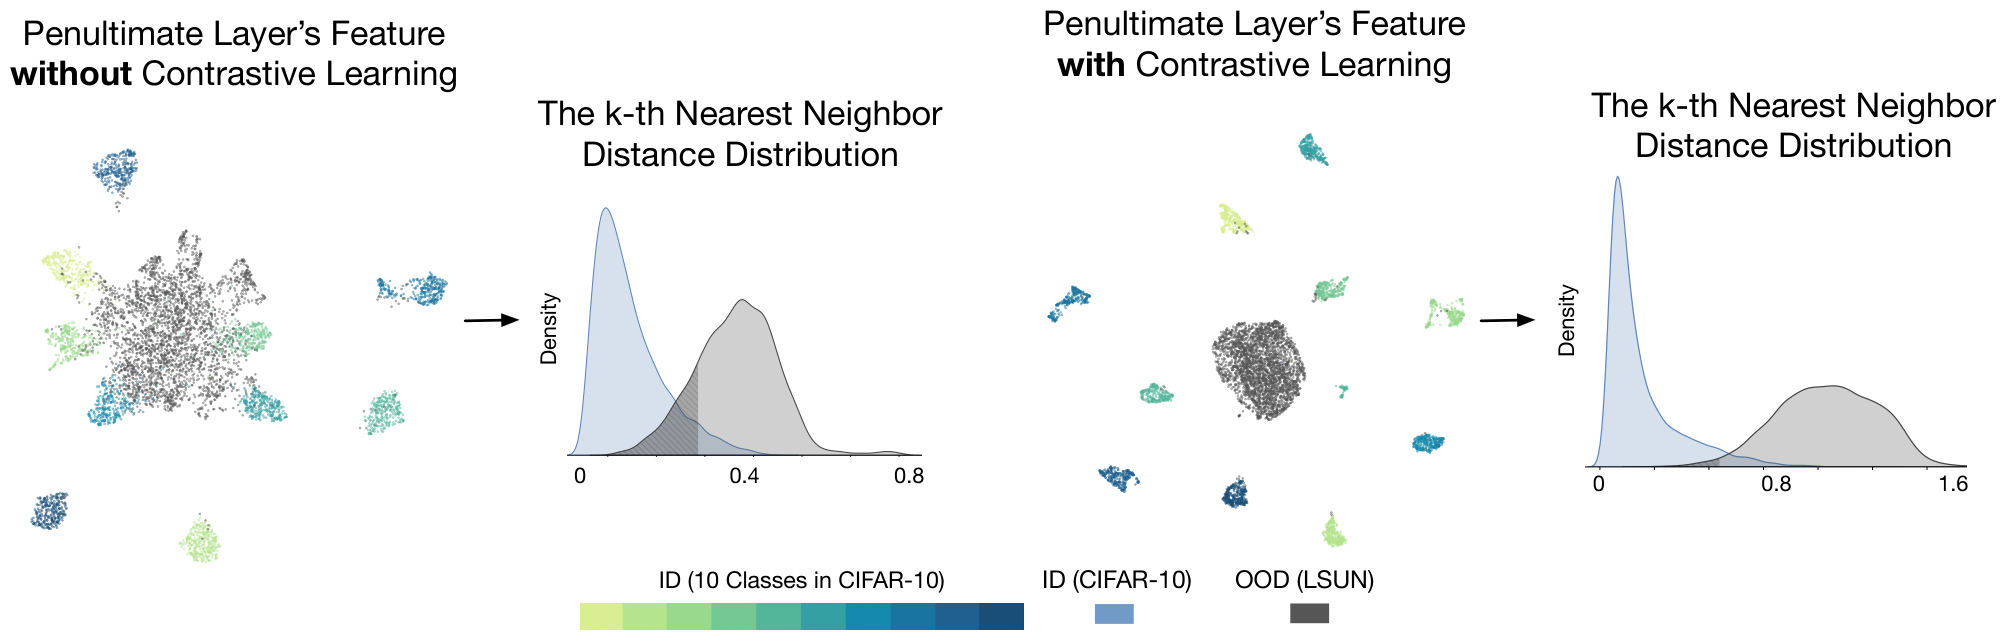
\includegraphics[width=\linewidth,height=0.32\textheight,keepaspectratio]{images/image-recognition/knnood_fig1_knn_distance.png}\\[0.2em]
      {\scriptsize CIFAR-10 (colours) vs LSUN scene images (grey), without and with contrastive training. Sun et al., ``Out-of-Distribution Detection with Deep Nearest Neighbors,'' ICML 2022, \href{https://arxiv.org/abs/2204.06507v3}{arXiv:2204.06507v3}, Figure~1.\par}
      \vspace{0.5em}
      {\centering\scriptsize
      \begin{tabular}{llcc}
        \toprule
        \textbf{Score} & \textbf{Training} & \textbf{FPR95} $\downarrow$ & \textbf{AUROC} $\uparrow$ \\
        \midrule
        MSP & CE & 66.95 & 81.99 \\
        Mahalanobis & CE & 87.43 & 55.47 \\
        $k$-NN & CE & 54.68 & 84.37 \\
        $k$-NN & SupCon & \textbf{38.47} & \textbf{90.91} \\
        \bottomrule
      \end{tabular}\par}
      \vspace{0.2em}
      {\scriptsize ResNet-50 on ImageNet-1K, cross-entropy (CE) or SupCon training, $k=1000$; mean over iNaturalist, SUN, Places, Textures. Sun et al., Table~4.\par}
  \end{columns}
\end{frame}

\begin{frame}{ViM: A Virtual Logit from the Feature Residual}
  \begin{columns}[T,onlytextwidth]
    \column{0.52\textwidth}
      \begin{itemize}\footnotesize\itemsep0.3em
        \item Feature scores ignore class identity; logit scores miss feature directions outside the span of the class weights. \textbf{Virtual-logit Matching (ViM)} (Wang et al., CVPR 2022) uses both.
        \item Figure notation: $x$ is the penultimate feature, shifted so the logits $l_i=w_i^{\top}x$ need no bias; $C$ classes.
        \item $P$: span of the top-$D$ eigenvectors of $X^{\top}X$ for training features $X$ (PCA-style); the residual $x^{P^\perp}$ is the part of $x$ outside $P$.
        \item Virtual logit $l_0=\alpha\|x^{P^\perp}\|$, with $\alpha$ set so its training mean equals the mean maximum logit:
        \[ \mathrm{ViM}(x)=\frac{e^{l_0}}{e^{l_0}+\sum_{i=1}^{C} e^{l_i}} \quad \text{(OOD if large)}. \]
        Ranking by ViM equals ranking by $l_0 + E(x)$: the energy plus the scaled residual norm.
      \end{itemize}
    \column{0.46\textwidth}
      \centering
      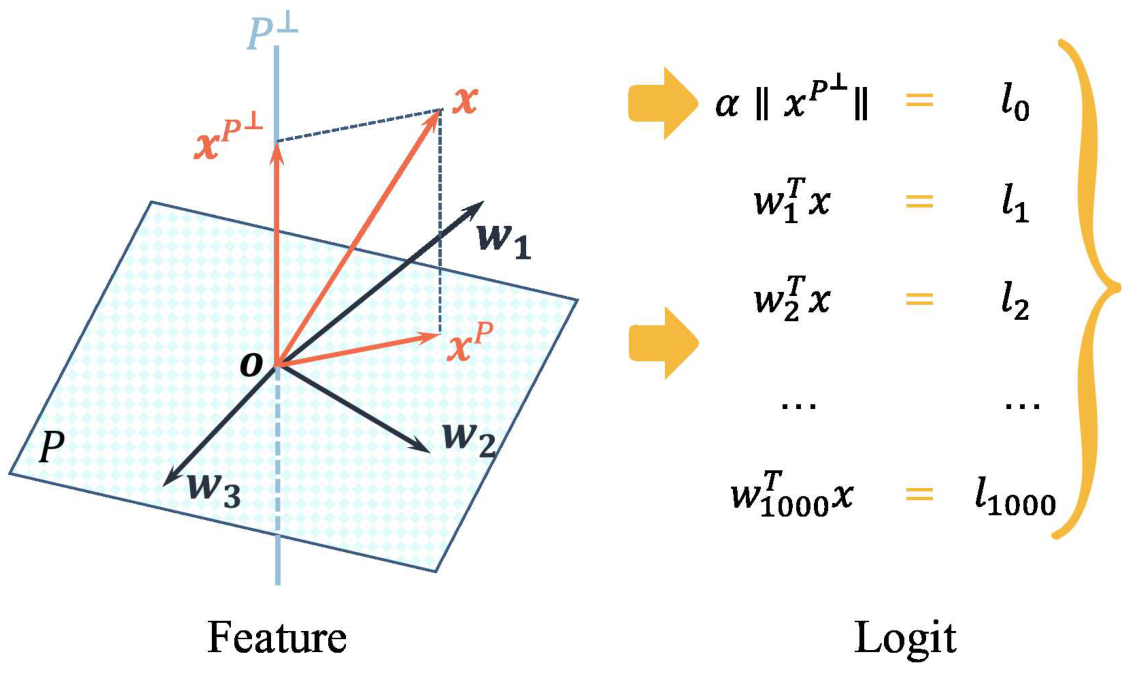
\includegraphics[width=\linewidth,height=0.36\textheight,keepaspectratio]{images/image-recognition/vim_fig3_feature_logit.png}\\[0.2em]
      {\scriptsize Feature and logit stages. Wang et al., ``ViM: Out-Of-Distribution with Virtual-logit Matching,'' CVPR 2022, \href{https://arxiv.org/abs/2203.10807v1}{arXiv:2203.10807v1}, Figure~3 (centre).\par}
      \vspace{0.6em}
      {\centering\scriptsize
      \begin{tabular}{lcc}
        \toprule
        \textbf{Score} & \textbf{BiT} & \textbf{ViT-B/16} \\
        \midrule
        MSP & 77.25 / 77.83 & 89.40 / 41.65 \\
        Energy & 78.48 / 79.68 & 94.90 / 22.43 \\
        Mahalanobis & 86.62 / 53.34 & 96.02 / 19.45 \\
        ViM & \textbf{90.91} / \textbf{41.46} & \textbf{96.23} / \textbf{18.07} \\
        \bottomrule
      \end{tabular}\par}
      \vspace{0.2em}
      {\scriptsize AUROC / FPR95 on ImageNet-1K, averaged over OpenImage-O, Textures, iNaturalist and ImageNet-O. BiT (Big Transfer): a ResNet-v2 trained on ImageNet-1K; the ViT is pre-trained on ImageNet-21K. Wang et al., Table~2.\par}
  \end{columns}
\end{frame}

\begin{frame}{Activation Shaping: ReAct, ASH, and SCALE}
  \begin{columns}[T,onlytextwidth]
    \column{0.58\textwidth}
      \begin{itemize}\footnotesize\itemsep0.3em
        \item All three edit the penultimate activations $h(x)\in\mathbb{R}^D$ (non-negative after the ReLU) before the last layer, then score with the energy $-E(x)$; no retraining.
        \item \textbf{ReAct} (rectified activations; Sun et al., NeurIPS 2021): $\bar h=\min(h(x),c)$ per unit, $c$ the 90th percentile of ID activations. OOD inputs push a few units to outsized values; clipping removes them. ID top-1: 75.08\% to 73.75\%.
        \item \textbf{ASH-S} (activation shaping; Djurisic et al., ICLR 2023): per image, zero activations below the image's 90th percentile, multiply the rest by $e^{s_1/s_2}$ ($s_1$, $s_2$: sums before and after pruning). ID top-1: 76.13\% to 74.98\%.
        \item \textbf{SCALE} (Xu et al., ICLR 2024): keep every activation and multiply all by $e^{r}$, $r=Q(h)/Q_p(h)$ (sum of all activations over the sum above the $p$-th percentile). The arg max, hence ID accuracy, is unchanged; they find ASH's gains come from scaling, while pruning hurts.
      \end{itemize}
    \column{0.40\textwidth}
      \centering
      \vspace{0.4em}
      {\centering\footnotesize
      \begin{tabular}{lcc}
        \toprule
        \textbf{Score} & \textbf{FPR95} $\downarrow$ & \textbf{AUROC} $\uparrow$ \\
        \midrule
        MSP & 66.95 & 81.99 \\
        Energy & 58.41 & 86.17 \\
        ReAct & 31.43 & 92.95 \\
        ASH-S & 22.80 & 95.12 \\
        SCALE & \textbf{20.05} & \textbf{95.71} \\
        \bottomrule
      \end{tabular}\par}
      \vspace{0.4em}
      {\scriptsize ResNet-50 on ImageNet-1K, averaged over iNaturalist, SUN, Places365 and Textures. Xu et al., ``Scaling for Training Time and Post-hoc Out-of-distribution Detection Enhancement,'' ICLR 2024, \href{https://proceedings.iclr.cc/paper_files/paper/2024/hash/46d943bc6a15a57c923829efc0db7c7a-Abstract-Conference.html}{proceedings.iclr.cc}, Table~7.\par}
      \vspace{0.6em}
      {\scriptsize On harder OOD classes that sit close to ImageNet's, a ResNet-50 with SCALE still has FPR95 59.76 (their Table~2).\par}
  \end{columns}
\end{frame}

\begin{frame}{Training-Time Fixes: Outlier Exposure and LogitNorm}
  \begin{columns}[T,onlytextwidth]
    \column{0.52\textwidth}
      \begin{itemize}\footnotesize\itemsep0.3em
        \item \textbf{Outlier Exposure (OE)} (Hendrycks et al., ICLR 2019): train on auxiliary outlier images $x'$, disjoint from the test OOD sets, with an extra loss weighted 0.5: the cross-entropy from $p(\cdot\mid x')$ to the uniform distribution. OSR protocols discourage such extra data by design (Yang et al.).
        \item \textbf{LogitNorm} (logit normalisation; Wei et al., ICML 2022): cross-entropy keeps inflating the logit norm $\|z\|$ on images already classified correctly, so confidence grows for ID and OOD alike. Train on normalised logits:
        \[ \mathcal{L} = -\log \frac{e^{z_y/(\tau\|z\|)}}{\sum_{k=1}^{K} e^{z_k/(\tau\|z\|)}} , \]
        with label $y$ and temperature $\tau$ (0.04 on CIFAR-10). CIFAR-10, MSP score, six OOD sets: FPR95 49.52 to 15.65 (WRN-40-2, a WideResNet); test accuracy 95.14\% vs 95.01\% (ResNet-34).
      \end{itemize}
    \column{0.46\textwidth}
      \centering
      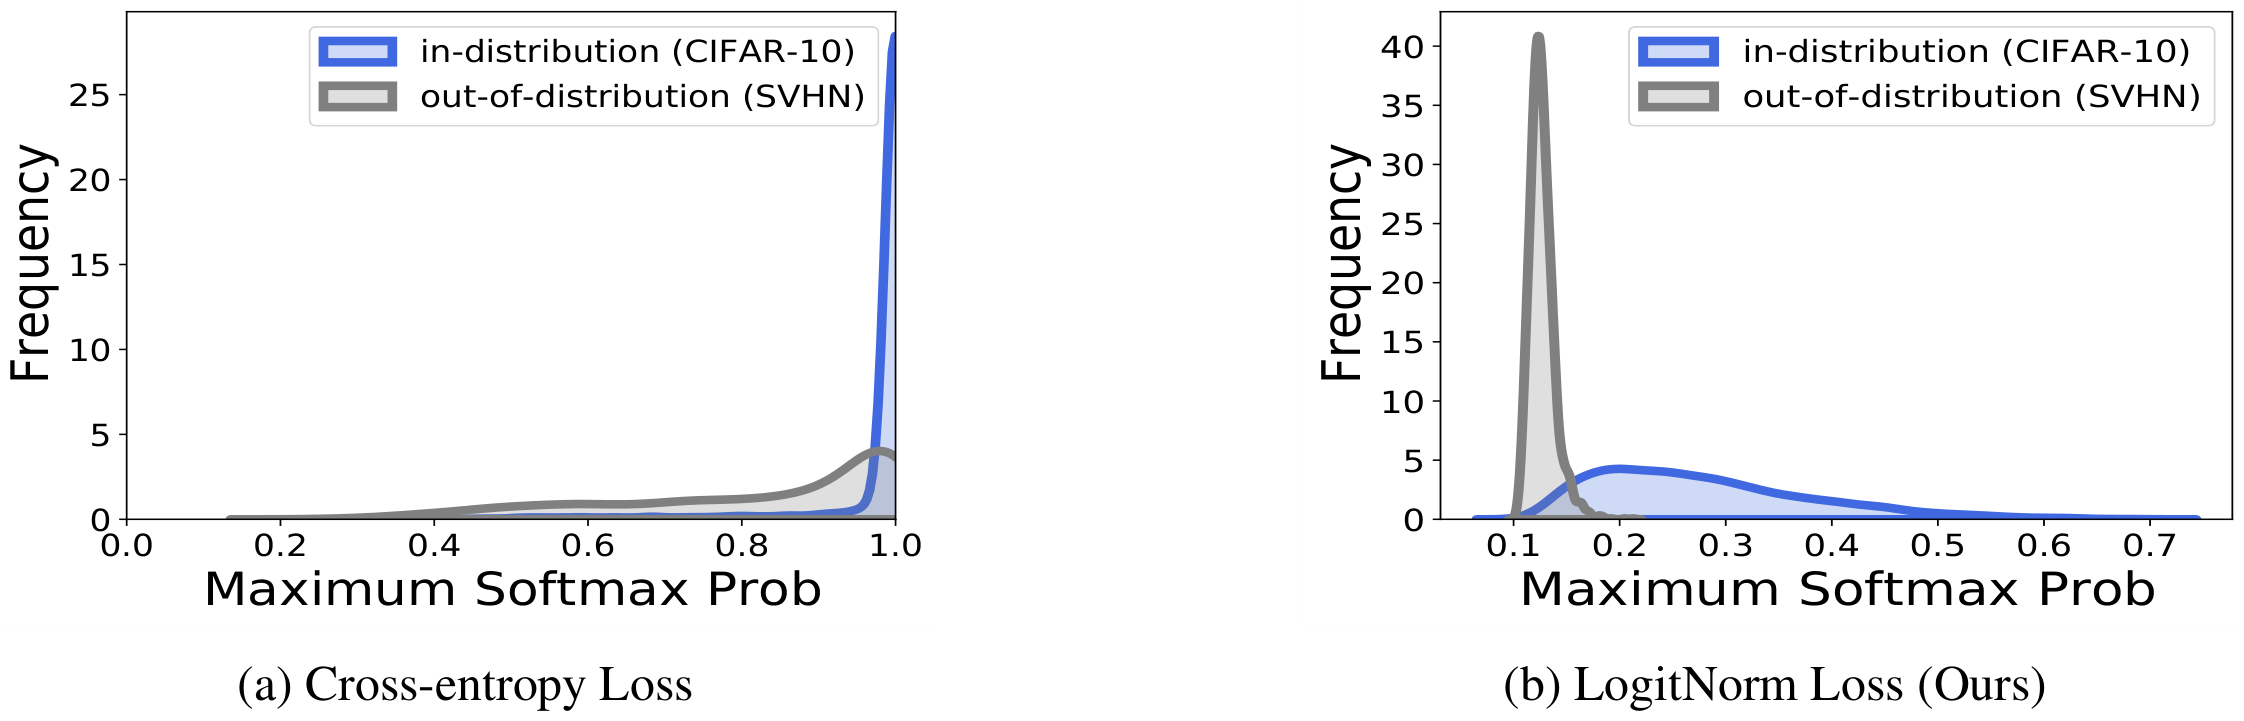
\includegraphics[width=\linewidth,height=0.30\textheight,keepaspectratio]{images/image-recognition/logitnorm_fig4_msp_histograms.png}\\[0.2em]
      {\scriptsize MSP histograms, CIFAR-10 (ID) vs SVHN (OOD), after cross-entropy (a) and LogitNorm (b) training. Wei et al., ``Mitigating Neural Network Overconfidence with Logit Normalization,'' ICML 2022, \href{https://arxiv.org/abs/2205.09310v2}{arXiv:2205.09310v2}, Figure~4.\par}
      \vspace{0.6em}
      {\centering\scriptsize
      \begin{tabular}{lcc}
        \toprule
        \textbf{ID data} & \textbf{MSP} & \textbf{MSP after OE} \\
        \midrule
        CIFAR-10 & 34.9 & 9.5 \\
        CIFAR-100 & 62.7 & 38.5 \\
        Places365 & 63.5 & 28.2 \\
        \bottomrule
      \end{tabular}\par}
      \vspace{0.2em}
      {\scriptsize FPR95 before and after OE fine-tuning. Hendrycks et al., ``Deep Anomaly Detection with Outlier Exposure,'' ICLR 2019, \href{https://arxiv.org/abs/1812.04606v3}{arXiv:1812.04606v3}, Table~1.\par}
  \end{columns}
\end{frame}
